\chapter{DNS (Domain Name System)}

\section{Definizione:}
\begin{boxDef}
\textbf{\textcolor{brown}{DNS:}} un'applicazione Internet che fornisce servizi ad altre applicazioni Internet. Introduce un nuovo livello di denominazione per le risorse Internet (oltre agli indirizzi IP) progettato per essere più intuitivo.
È un esempio di sistema distribuito su scala globale che funziona molto bene, ha superato di gran lunga le aspettative in termini di scalabilità e ha superato la prova del tempo.
\end{boxDef}

\section{Host identifiers}
Ogni host in un rete necessita di almeno un IP, ma può avere anche più \textbf{hostname}.
\begin{boxDef}
\textbf{\textcolor{brown}{Hostname:}} è una stringa \textbf{alfanumerica} di \textbf{255} caratteri, formata da \textbf{label}, ognuno divisa da un punto. Molto più facile da ricordare rispetto a un indirizzo IP e comoda per ambienti dinamici, infatti, si può usare lo stesso hostname anche quando l'ip cambia.
\end{boxDef}
Il vero hostname è chiamato \textbf{canonico}, da cui si possono derivare degli \textbf{alias}.

\begin{figure}[!htb]
    \centering
    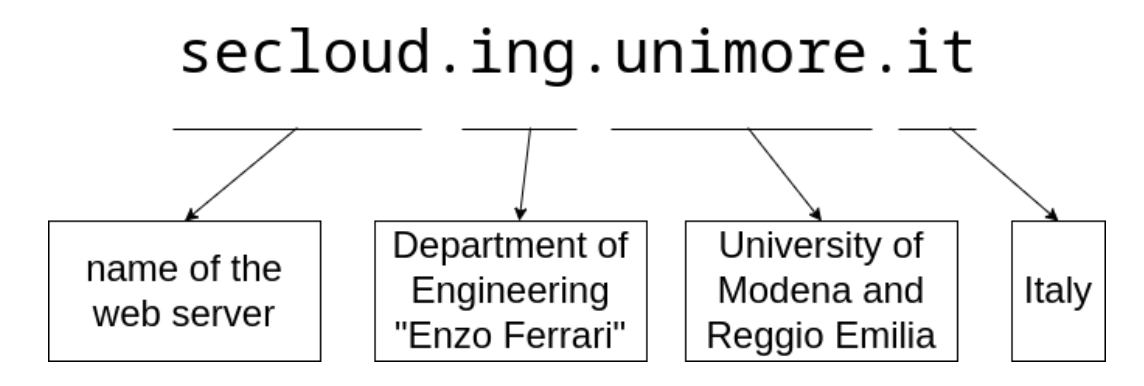
\includegraphics[width=0.6\linewidth]{Images/DNS/hostname.png}
    \caption{Esempio di Hostname canonico.}
\end{figure}

Ogni label rappresenta un livello di gerarchia diverso.
Ovviamente, implementando un sistema di questo tipo, deve essere anche creato un modo per convertire gli hostname nel loro IP e vicevarsa. 

\begin{figure}[!htb]
    \centering
    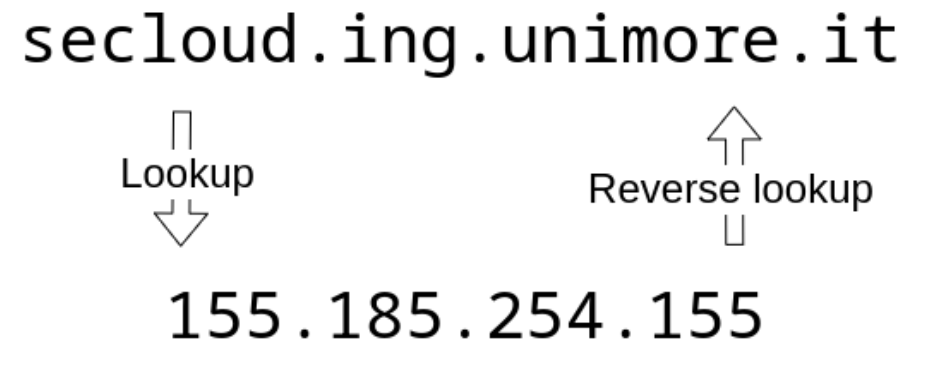
\includegraphics[width=0.4\linewidth]{Images/DNS/lookup.png}
    \caption{Lookup e reverse lookup.}
\end{figure}

All'inizio, venivano usati dei file contenti ogni IP col proprio hostname, ma col crescere dei file si è cercato un modo più scalabile e dinamico, il DNS.

\section{Name Servers}
Divisi in diversi livelli:
\begin{itemize}
    \item \textbf{Root name server:} 13 server, denominati dalla A alla M. Sono distribuiti in ambienti altamente controllati e protetti e gestiti da 12 organizzazioni indipendenti. Inoltre, sono \textbf{autorevole}, devono sapere tutti gli IP dei TLD name server.
    \item \textbf{TLD (Top Level Domain) name server:} deve fornire almeno due name server diversi che siano autorevoli per la sua zona. Tutti conosco gli IP dei SLD name server.
    \item \textbf{SLD (Second Level Domain) name server:} deve fornire almeno due name server diversi che siano autorevoli per la sua zona. Conoscono tutti gli IP dei name server più sotto.
    \item \textbf{Local name server.}
\end{itemize}

\subsection{Resource Records}
In un nameserver, i dati vengono memorizzati come un insieme di \textbf{resources records}. I nameserver consentono meccanismi di ricerca IP diretti e inversi.
Ogni record di risorse ha 6 campi:

\begin{figure}[!htb]
    \centering
    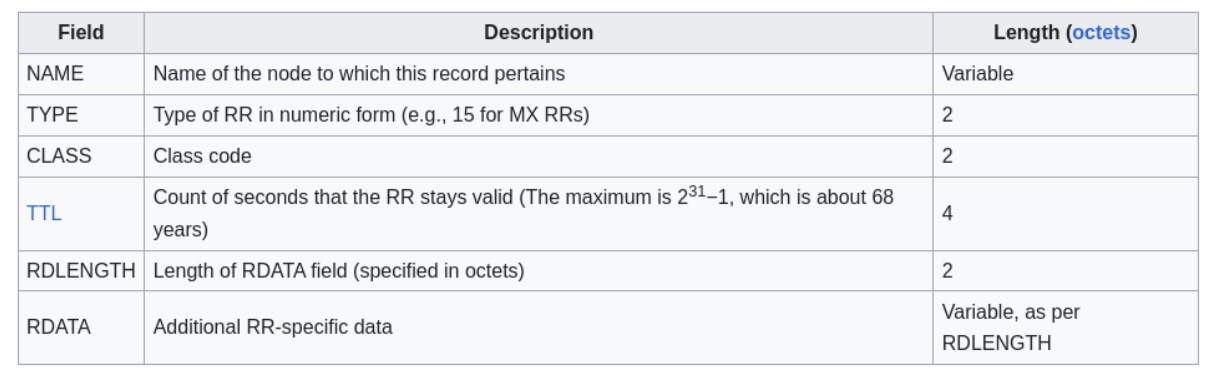
\includegraphics[width=0.8\linewidth]{Images/DNS/Records.png}
    \caption{Campi di un resource record.}
\end{figure}

Alcuni record comuni sono:
\begin{itemize}
    \item \textbf{A:} contiene un indirizzo ipv4 associato a un Fully Qualified Domain Name (FQDN).
    \item \textbf{AAAA:} contiene un indirizzo ipv6 associato a un Fully Qualified Domain Name (FQDN).
    \item \textbf{NS:} memorizza il FQDN del name server autorevole per una determinata zona.
    \item \textbf{NX:} memorizza il FQDN dei server di posta che riceveranno le email per i destinatari di un determinato dominio.
    \item \textbf{CNAME:} contiene il nome canonico di un determinati alias.
    \item \textbf{PRT:} contiene il CNAME associato a un determinati IP.
    \item \textbf{SOA:} contiene parametri di configurazione per la zona.
    \item \textbf{TXT:} associa a una FQDN una stringa arbitraria.
\end{itemize}

Si possono vedere direttamente le query con il comando \textbf{dig}:
\begin{bashbox}
ddig [RR_type] FQDN [@nameserver]
\end{bashbox}
Per esempio:
\begin{bashbox}
ddig A www.unimore.it @8.8.8.8
dig MX unimore.it @155.185.1.2
dig SOA unimore.it @155.155.1.2
dig NS unimore.it @193.0.14.129
\end{bashbox}

\newpage
\subsection{Risoluzione dei nomi in modo distribuito}
Nessun server DNS conosce tutti i valori di tutti i \textbf{record RR} dell'intero Internet, è necessaria una qualche forma di \textbf{cooperazione}.
Il DNS utilizza un approccio client-server:
\begin{enumerate}
    \item Il client avvia il processo di ricerca inviando una query a un name server, di solito si tratta di quello locale configurato in ciascun dispositivo. 
    \item Se conosce la risposta, la fornisce direttamente al client.
    \item Se non conosce la risposta deve chiederla a un altro name server.
\end{enumerate}
Le query possono essere \textbf{ricorsive}, dove ogni name server chiede in automatico a un altro name server, oppure \textbf{iterative} dove sarà l'utente a interrogare più name server.
Ogni name server possiede una cache con alcune risposte, alla scadenza del loro \textbf{TTL} verranno eliminate.

\section{Pacchetto DNS}
Facendo parte del livello applicativo, oltre agli header del protocollo IP e del protocollo UDP, al pacchetto viene aggiunto quello del protocollo DNS.

\begin{figure}[!htb]
    \centering
    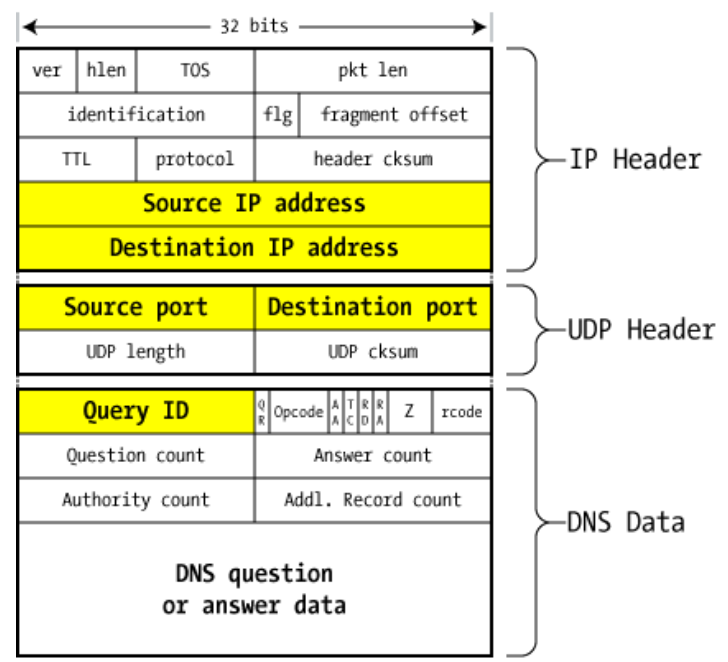
\includegraphics[width=0.5\linewidth]{Images/DNS/Pacchetto_DNS.png}
    \caption{Campi di un resource record.}
\end{figure}

In particolare:
\begin{itemize}
    \item \textbf{Query ID:} identificatore univoco creato nel pacchetto di query e ripetuto dal server nella risposta.
    \item \textbf{QR (Query / Response):} 0 se è una query, 1 se è una risposta.
    \item \textbf{Opcode:} per il tipo di query, standard è 0.
    \item \textbf{AA (Authorative Answer):} 1 se una riposta è autorevole.
    \item \textbf{TC (Trunkated):} la riposta non stava nel pacchetto UDP, sarà necessario fare una nuova richiesta con un segmento TCP.
    \item \textbf{RD (Recursion Desired):} 1 se si vuole fare una query ricorsiva, 0 altrimenti.
    \item \textbf{RA (Recursion Available):} 1 se si può fare una query ricorsiva, 0 altrimenti.
    \item \textbf{Z:} non usato, deve essere 0.
    \item \textbf{rcode:} codice di riposta del server, successo o fallimento.
    \item \textbf{Question record count.} 
    \item \textbf{Answer/Authorative/Additional record count:} inseriti dal server.
    \item \textbf{NDS question:} campo che contiene i dati della richiesta/risposta.
\end{itemize}
